\documentclass[12pt,twoside,a4paper]{report}
\usepackage[a4paper,width=150mm,top=25mm,bottom=25mm,bindingoffset=6mm]{geometry}

\usepackage[utf8x]{inputenc}
\usepackage[slovak]{babel}
\usepackage{palatino,verbatim}

% Balicek pre priamu rec - \say
\usepackage{dirtytalk}

% Balicek "alltt" je to iste ako "verbatim" mod, ale navyse podporuje aj formatovacie znacky textu
\usepackage{alltt}

% Obrazky
\usepackage{graphicx}
\graphicspath{ {obr/} }

% Cislovanie obrazkov a tabuliek
\usepackage{chngcntr}
%Cisluj obrazky nezavisle od cisla kapitol/podkapitol
\counterwithout{figure}{subsection}
\counterwithout{table}{subsection}

% Referencovanie kapitol/sekcii/... podľa ich nadpisu
\usepackage{nameref}

% Tabulky s viacriadkovymi bunkami a zlucenymi bunkami
% Tabulky generujem naastrojom "http://www.tablesgenerator.com/"
\usepackage{booktabs}
\usepackage{multirow}
% LaTeX ma problemy s prikazmi cline a cmidrule, ked je babel nastaveny na slovencinu/cestinu, kvoli definicii pomlcky
% NAMIESTO POMLCKY POUZI ZNAK ZNAMIENKA MINUS "−" (plati hlavne v nazvoch nadpisov a labelov)
\usepackage{etoolbox}
\preto\tabular{\shorthandoff{-}}

%Uloz obrazok tam, kde je deklarovany
%\usepackage[subsection]{placeins}

\newcommand\sktxt[1]{\foreignlanguage{slovak}{#1}}

\begin{document}
\pagenumbering{arabic}

\setcounter{chapter}{1}
\chapter*{Internet Peering}
\paragraph{}
Andrej Šišila, Marián Vachalík

\tableofcontents

\newpage
\section{Topológia}
\paragraph{}
Budeme konfigurovať smerovacie protokoly BGP a IS-IS na topológií, ktorá je znázornená na obrázku \ref{fig:bgp_isis_topo}. Vrámci autonómnych systémov sme konfigurovali smerovacie protokoly IS-IS a BGP (iBGP). Medzi autonómnymi systémami sme konfigurovali len BGP (eBGP). IP adresácia je uvedená v tabuľke \ref{tab:ip_adresacia} a dopĺňa grafické znázornenie topológie na obrázku \ref{fig:bgp_isis_topo}. Sieť medzi smerovačmi R1 a R5 nemá mať masku \say{/48} ale \say{/30}.

\begin{figure}[!htbp]
\centering
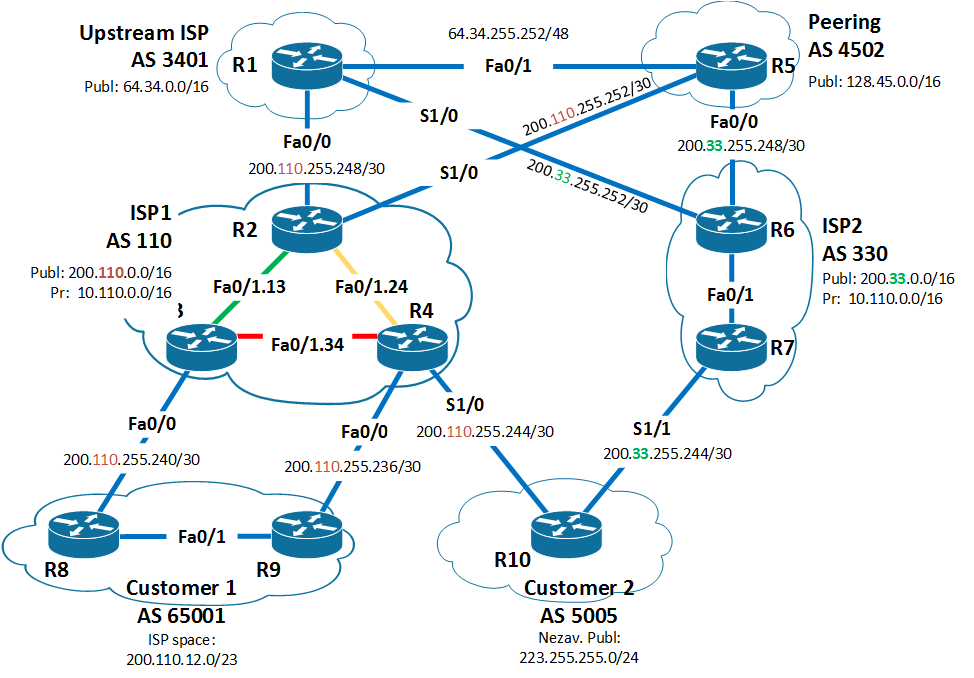
\includegraphics[width=14cm,keepaspectratio]{bgp_isis_topo}
\caption{Topológia BGP}
\label{fig:bgp_isis_topo}
\end{figure}



\begin{table}[!htbp]
\centering
\caption{IP adresácia}
\label{tab:ip_adresacia}
\begin{tabular}{|c|l|l|l|}
\hline
\textbf{Smerovač}    & \multicolumn{1}{c|}{\textbf{Rozhranie}} & \multicolumn{1}{c|}{\textbf{IP adresa}} & \multicolumn{1}{c|}{\textbf{Maska}} \\ \hline
\multirow{5}{*}{R1}  & Fa0/0                                   & 200.110.255.249                         & 255.255.255.252                     \\ \cline{2-4} 
                     & Fa0/1                                   & 64.34.255.253                           & 255.255.255.252                     \\ \cline{2-4} 
                     & S1/0                                    & 200.33.255.253                          & 255.255.255.252                     \\ \cline{2-4} 
                     & Lo0                                     & 10.255.255.1                            & 255.255.255.0                       \\ \cline{2-4} 
                     & Lo100                                   & 64.34.1.1                               & 255.255.255.128                     \\ \hline
\multirow{6}{*}{R2}  & Fa0/0                                   & 200.110.255.250                         & 255.255.255.252                     \\ \cline{2-4} 
                     & Fa0/1.23                                & 10.110.23.2                             & 255.255.255.0                       \\ \cline{2-4} 
                     & Fa0/1.24                                & 10.110.24.2                             & 255.255.255.0                       \\ \cline{2-4} 
                     & S1/0                                    & 200.110.255.253                         & 255.255.255.252                     \\ \cline{2-4} 
                     & Lo0                                     & 10.255.255.2                            & 255.255.255.0                       \\ \cline{2-4} 
                     & Lo100                                   & 200.110.0.2                             & 255.255.255.128                     \\ \hline
\multirow{5}{*}{R3}  & Fa0/0                                   & 200.110.255.241                         & 255.255.255.252                     \\ \cline{2-4} 
                     & Fa0/1.23                                & 10.110.23.3                             & 255.255.255.0                       \\ \cline{2-4} 
                     & Fa0/1.34                                & 10.110.34.3                             & 255.255.255.0                       \\ \cline{2-4} 
                     & Lo0                                     & 10.255.255.3                            & 255.255.255.0                       \\ \cline{2-4} 
                     & Lo100                                   & 200.110.0.133                           & 255.255.255.128                     \\ \hline
\multirow{6}{*}{R4}  & Fa0/0                                   & 200.110.255.237                         & 255.255.255.252                     \\ \cline{2-4} 
                     & Fa0/1.24                                & 10.110.24.4                             & 255.255.255.0                       \\ \cline{2-4} 
                     & Fa0/1.34                                & 10.110.34.4                             & 255.255.255.0                       \\ \cline{2-4} 
                     & S1/0                                    & 200.110.255.245                         & 255.255.255.252                     \\ \cline{2-4} 
                     & Lo0                                     & 10.255.255.4                            & 255.255.255.0                       \\ \cline{2-4} 
                     & Lo100                                   & 200.110.1.4                             & 255.255.255.128                     \\ \hline
\multirow{5}{*}{R5}  & Fa0/0                                   & 200.33.255.249                          & 255.255.255.252                     \\ \cline{2-4} 
                     & Fa0/1                                   & 10.100.15.2                             & 255.255.255.252                     \\ \cline{2-4} 
                     & S1/0                                    & 200.110.255.254                         & 255.255.255.252                     \\ \cline{2-4} 
                     & Lo0                                     & 10.255.255.5                            & 255.255.255.0                       \\ \cline{2-4} 
                     & Lo100                                   & 128.45.5.5                              & 255.255.255.128                     \\ \hline
\multirow{5}{*}{R6}  & Fa0/0                                   & 200.33.255.250                          & 255.255.255.252                     \\ \cline{2-4} 
                     & Fa0/1                                   & 10.110.67.6                             & 255.255.255.0                       \\ \cline{2-4} 
                     & S1/0                                    & 200.33.255.254                          & 255.255.255.252                     \\ \cline{2-4} 
                     & Lo0                                     & 10.255.255.6                            & 255.255.255.0                       \\ \cline{2-4} 
                     & Lo100                                   & 200.33.6.6                              & 255.255.255.128                     \\ \hline
\multirow{4}{*}{R7}  & Fa0/1                                   & 10.110.67.7                             & 255.255.255.0                       \\ \cline{2-4} 
                     & S1/1                                    & 200.33.255.245                          & 255.255.255.252                     \\ \cline{2-4} 
                     & Lo0                                     & 10.255.255.7                            & 255.255.255.0                       \\ \cline{2-4} 
                     & Lo100                                   & 200.33.7.7                              & 255.255.255.128                     \\ \hline
\multirow{4}{*}{R8}  & Fa0/0                                   & 200.110.255.242                         & 255.255.255.252                     \\ \cline{2-4} 
                     & Fa0/1                                   & 10.110.89.8                             & 255.255.255.0                       \\ \cline{2-4} 
                     & Lo0                                     & 10.255.255.8                            & 255.255.255.0                       \\ \cline{2-4} 
                     & Lo100                                   & 200.110.12.8                            & 255.255.255.128                     \\ \hline
\multirow{4}{*}{R9}  & Fa0/0                                   & 200.110.255.238                         & 255.255.255.252                     \\ \cline{2-4} 
                     & Fa0/1                                   & 10.110.89.9                             & 255.255.255.0                       \\ \cline{2-4} 
                     & Lo0                                     & 10.255.255.9                            & 255.255.255.0                       \\ \cline{2-4} 
                     & Lo100                                   & 200.110.13.9                            & 255.255.255.128                     \\ \hline
\multirow{4}{*}{R10} & S1/0                                    & 200.110.255.246                         & 255.255.255.252                     \\ \cline{2-4} 
                     & S1/1                                    & 200.33.255.246                          & 255.255.255.252                     \\ \cline{2-4} 
                     & Lo0                                     & 10.255.255.10                           & 255.255.255.0                       \\ \cline{2-4} 
                     & Lo100                                   & 223.255.255.10                          & 255.255.255.128                     \\ \hline
\end{tabular}
\end{table}


% Novu kapitolu davam na novu stranu, lebo bez toho mi zobrazuje tabulku v dalsej kapitole, kde ale tabulka nepatri.
\newpage

\section{Úlohy}
\subsection{Použiť IGP IS−IS (L2 only) single area dizajn, priame p2p prepojenia}
\subsection{Zabezpečiť plnú konektivitu prostredníctvom iBGP alebo eBGP protokolov pre zákaznícké a internetové smerovacie záznamy}
\subsection{Distribúcia internetových statických smerovacích záznamov z AS3401, AS4502 a zákaznických smerovacích záznamov z AS65001, AS5005, AS330}
\subsection{Sumarizácia}


\subsubsection{Popis}
\paragraph{}
V celej topológií používame smerovací protokol BGP. Vnútri všetkých autonómnych systémov navyše používame smerovací protokol IS-IS. Subrozhranie “.13” (VLAN 13) sme premenovali na “.23” (VLAN 23), lebo sieť je medzi smerovačmi R2 a R3 (23), a nie medzi R1 a R3 (13).

\paragraph{}
Najprv sme linky medzi autonómnymi systémami šírili cez IS-IS. Neskôr sa toto ukázalo ako nevhodné riešenie, pretože \say{flappovacie} linky u zákazníkov môžu spôsobiť nestabilitu siete. Preto boli rozhrania medzi AS odstranené z IS-IS príkazmi uvedenými nižšie.

\noindent
{\fontfamily{qcr}\selectfont
\begin{small}
\begin{alltt}
int <nazov_interfaceu>
  no ip router isis
router isis
  no passive-interface <nazov_interfaceu>
  no redistribute-connected
\end{alltt}
\end{small}
}

\paragraph{}
Na smerovačoch sme vytvorili dve virtuálne rozhrania: Loopback0 a Loopback100. Loopback0 mal IP adresu v tvare \say{10.255.255.X} s maskou \say{/32}, kde X je číslo smerovača. Router-ID sme nastavili na IP adresu rozhrania Loopback0. V rámci BGP sme ho nastavovali príkazom \say{bgp router-id 10.255.255.X}. Pokiaľ sa Router ID v BGP nenastaví hneď na začiatku, jeho zmena spôsobí rozpad BGP spojenia, ktoré sa po chvíli (rádovo v desiatkach sekúnd) obnoví.

\paragraph{}
Loopback100 mal IP adresu z verejného rozsahu príslušnej autonómnej oblasti s maskou \say{/25}. Verejné adresné rozsahy na Loopback100 rozhraniach sme sumarizovali pre každú AS príkazom \say{aggregate-address}. S AS 65001 vznikol problém so sumarizáciou ich verejného rozsahu na smerovačoch R3 a R4, lebo, lebo \say{Customer 1} (AS 65001) mal používal podrozsah verejných adries \say{ISP1} (AS 110). Ak by sme na R3 a R4 vykonali sumarizáciu verejných rozsahov pre Loopback100 v AS 110, spôsobilo by to, že \say{next-hop} adresa pre Loopback100 v AS 65001 by bol \say{Null0} t.j. paket by bol zahodený. Na R4 sme sumarizáciu nerobili, pretože keby vypadla linka medzi R2 a R3, do AS 65001 by sme išli cez R4, a pokiaľ by mal R4 spomenutú sumárnu cestu, vznikol by ten istý problém s konektivitou.

\paragraph{}
V rámci BGP sme každému smerovaču nakonfigurovali siete, s ktorými susedí resp. na ktoré je priamo pripojený príkazom \say{neighbor}. Podľa toho, či sa susediaca sieť nachádza v AS s rovnakým číslom ako je ASN daného smerovača, použije sa iBGP, inak sa použije eBGP. 

\paragraph{}
Siete obidvoch Loopback rozhraní sme ohlasovali príkazom \say{network} v rámci BGP. Potom sme pre ne použili príkaz \say{update-source}, ktorý slúži na prepísanie zdrojovej IP adresy na Loopback0. Keďže sme Loopback0 ohlásili príkazom \say{network}, susediace smerovače mu budú môcť odpovedať. Zdrojová adresa sa potom použije na otvorenie BGP spojenia medzi susednými smerovačmi. Loopback0 používame aj kvôli tomu, že bude vždy zapnutý, takže BGP spojenie bude stále aktívne.

\paragraph{}
Pokiaľ boli v AS viac ako dva smerovače, museli sme pridať príkaz \say{next-hop-self}, aby sme zaistili konektivitu medzi AS. Príkaz \say{next-hop-self} sa používa, keď sa BGP smerovač v jednom AS dozvie o ceste z iného AS cez eBGP a dá o tejto ceste vedieť zvyšným iBGP smerovačom v rámci svojho AS. Aby mohol iBGP smerovač získať konektivitu do tejto siete, použijeme na eBGP príkaz \say{next-hop-self}, ktorý namiesto toho, aby preposielal prefix s \say{next-hop} adresou zo siete medzi operátormi, prepíše \say{next-hop} adresu na svoj Loopback0. iBGP smerovač tak získa konektivitu do danej siete cez hraničný eBGP smerovač vo svojej oblasti. Keby sme tak neurobili, iBGP smerovač by sa nemohol dostať do siete v susednom AS, keď k nej nemá eBGP spojenie a z dôvodu bezpečnosti sme linky medzi AS neohlasovali príkazom \say{network}.


\subsubsection{Konfigurácia}

\noindent
{\fontfamily{qcr}\selectfont
\begin{small}
\begin{alltt}
R1
ena
conf t
hostname R1
no ip domain-lookup
username admin privil 15 secret admin
line con 0
  login local
  logging syn
  exec-time 120
line vty 0 15
  privilege level 15
  no login
int f0/0
  ip addr 200.110.255.249 255.255.255.252
  no shut
int f0/1
  ip addr 64.34.255.253 255.255.255.252
  no shut
int s1/0
  ip addr 200.33.255.253 255.255.255.252
  no shut
int lo0
  ip addr 10.255.255.1 255.255.255.255
  no shut
int lo100
  ip addr 64.34.1.1 255.255.255.128
  no shut
router bgp 3401
  bgp router-id 10.255.255.1
  neighbor 64.34.255.254 remote-as 4502
  neighbor 200.33.255.254 remote-as 330
  neighbor 200.110.255.250 remote-as 110
  network 10.255.255.1 mask 255.255.255.255
  network 64.34.1.0 mask 255.255.255.128
  aggregate-address 64.34.0.0 255.255.0.0 summary-only
  no auto-summary
  no sync
  bgp log-neighbor-changes



R2
ena
conf t
hostname R2
no ip domain-lookup
username admin privil 15 secret admin
line con 0
  login local
  logging syn
  exec-time 120
line vty 0 15
  privilege level 15
  no login
int f0/0
  ip addr 200.110.255.250 255.255.255.252
  no shut
int f0/1
  no ip add
  isis network point-to-point
  no sh
int f0/1.23
  encap dot1q 23
  ip addr 10.110.23.2 255.255.255.0
  ip router isis
int f0/1.24
  encap dot1q 24
  ip addr 10.110.24.2 255.255.255.0
  ip router isis
int s1/0
  ip addr 200.110.255.253 255.255.255.252
  no shut
int lo0
  ip addr 10.255.255.2 255.255.255.255
  ip router isis
  no shut
int lo100
  ip addr 200.110.0.2 255.255.255.128
  ip router isis
  no shut
router isis
  net 49.0001.0102.5525.5002.00
  passive-interface lo0
  passive-interface lo100
  redistribute static
  is-type level-2
  metric-style wide
  exit
router bgp 110
  bgp router-id 10.255.255.2
  neighbor 10.255.255.3 remote-as 110
  neighbor 10.255.255.3 update-source lo0
  neighbor 10.255.255.3 next-hop-self
  neighbor 10.255.255.4 remote-as 110
  neighbor 10.255.255.4 update-source lo0
  neighbor 10.255.255.4 next-hop-self
  neighbor 200.110.255.249 remote-as 3401
  neighbor 200.110.255.254 remote-as 4502
  network 10.255.255.2 mask 255.255.255.255
  network 200.110.0.0 mask 255.255.255.128
  aggregate-address 200.110.0.0 255.255.0.0 summary-only
  no auto-summary
  no sync
  bgp log-neighbor-changes



R3
ena
conf t
hostname R3
no ip domain-lookup
username admin privil 15 secret admin
line con 0
  login local
  logging syn
  exec-time 120
line vty 0 15
  privilege level 15
  no login
int f0/0
  ip addr 200.110.255.241 255.255.255.252
  no shut
int f0/1
  no ip addr
  isis network point-to-point
  no shut
int f0/1.23
  encap dot1q 23
  ip addr 10.110.23.3 255.255.255.0
  ip router isis
int f0/1.34
  encap dot1q 34
  ip addr 10.110.34.3 255.255.255.0
  ip router isis
int lo0
  ip addr 10.255.255.3 255.255.255.255
  ip router isis
  no shut
int lo100
  ip addr 200.110.0.133 255.255.255.128
  ip router isis
  no shut
router isis
  net 49.0001.0102.5525.5003.00
  passive-interface lo0
  passive-interface lo100
  redistribute static
  is-type level-2
  metric-style wide
  exit
router bgp 110
  bgp router-id 10.255.255.3
  neighbor 10.255.255.2 remote-as 110
  neighbor 10.255.255.2 update-source lo0
  neighbor 10.255.255.2 next-hop-self
  neighbor 10.255.255.4 remote-as 110
  neighbor 10.255.255.4 update-source lo0
  neighbor 10.255.255.4 next-hop-self
  neighbor 200.110.255.242 remote-as 65001
  network 10.255.255.3 mask 255.255.255.255
  network 200.110.0.128 mask 255.255.255.128
  no auto-summary
  no sync
  bgp log-neighbor-changes




R4
ena
conf t
hostname R4
no ip domain-lookup
username admin privil 15 secret admin
line con 0
  login local
  logging syn
  exec-time 120
line vty 0 15
  privilege level 15
  no login
int f0/0
  ip addr 200.110.255.237 255.255.255.252
  no shut
int f0/1
  no ip addr
  isis network point-to-point
  no sh
int f0/1.24
  encap dot1q 24
  ip addr 10.110.24.4 255.255.255.0
  ip router isis
int f0/1.34
  encap dot1q 34
  ip addr 10.110.34.4 255.255.255.0
  ip router isis
int s1/0
  ip addr 200.110.255.245 255.255.255.252
  no shut
int lo0
  ip addr 10.255.255.4 255.255.255.255
  ip router isis
  no shut
int lo100
  ip addr 200.110.1.4 255.255.255.128
  ip router isis
  no shut
router isis
  net 49.0001.0102.5525.5004.00
  passive-interface lo0
  passive-interface lo100
  redistribute static
  is-type level-2
  metric-style wide
  exit
router bgp 110
  bgp router-id 10.255.255.4
  neighbor 10.255.255.2 remote-as 110
  neighbor 10.255.255.2 update-source lo0
  neighbor 10.255.255.2 next-hop-self
  neighbor 10.255.255.3 remote-as 110
  neighbor 10.255.255.3 update-source lo0
  neighbor 10.255.255.3 next-hop-self
  neighbor 200.110.255.238 remote-as 65001
  neighbor 200.110.255.246 remote-as 5005
  network 10.255.255.4 mask 255.255.255.255
  network 200.110.1.0 mask 255.255.255.128
  no auto-summary
  no sync
  bgp log-neighbor-changes


R5
ena
conf t
hostname R5
no ip domain-lookup
username admin privil 15 secret admin
line con 0
  login local
  logging syn
  exec-time 120
line vty 0 15
  privilege level 15
  no login
int f0/0
  ip addr 200.33.255.249 255.255.255.252
  no shut
int f0/1
  ip addr 64.34.255.254 255.255.255.252
  no shut
int s1/0
  ip addr 200.110.255.254 255.255.255.252
  no shut
int lo0
  ip addr 10.255.255.5 255.255.255.255
  no shut
int lo100
  ip addr 128.45.5.5 255.255.255.128
  no shut
router bgp 4502
  bgp router-id 10.255.255.5
  neighbor 200.33.255.250 remote-as 330
  neighbor 200.110.255.253 remote-as 110
  neighbor 64.34.255.253 remote-as 3401
  network 10.255.255.5 mask 255.255.255.255
  network 128.45.5.0 mask 255.255.255.128
  aggregate-address 128.45.0.0 255.255.0.0 summary-only
  no auto-summary
  no sync
  bgp log-neighbor-changes




R6
ena
conf t
hostname R6
no ip domain-lookup
username admin privil 15 secret admin
line con 0
  login local
  logging syn
  exec-time 120
line vty 0 15
  privilege level 15
  no login
int f0/0
  ip addr 200.33.255.250 255.255.255.252
  no shut
int f0/1
  ip addr 10.110.67.6 255.255.255.0
  ip router isis
  isis network point-to-point
  no shut
int s1/0
  ip addr 200.33.255.254 255.255.255.252
  no shut
int lo0
  ip addr 10.255.255.6 255.255.255.255
  ip router isis
  no shut
int lo100
  ip add 200.33.6.6 255.255.255.128
  ip router isis
router isis
  net 49.0001.0102.5525.5006.00
  passive-interface lo0
  passive-interface lo100
  redistribute static
  is-type level-2
  metric-style wide
  exit
router bgp 330
  bgp router-id 10.255.255.6
  neighbor 10.255.255.7 remote-as 330
  neighbor 10.255.255.7 update-source lo0
  neighbor 10.255.255.7 next-hop-self
  neighbor 200.33.255.253 remote-as 3401
  neighbor 200.33.255.249 remote-as 4502
  network 10.255.255.6 mask 255.255.255.255
  network 200.33.6.0 mask 255.255.255.128
  aggregate-address 200.33.0.0 255.255.0.0 summary-only
  no auto-summary
  no sync
  bgp log-neighbor-changes



R7
ena
conf t
hostname R7
no ip domain-lookup
username admin privil 15 secret admin
line con 0
  login local
  logging syn
  exec-time 120
line vty 0 15
  privilege level 15
  no login
int f0/1
  ip addr 10.110.67.7 255.255.255.0
  ip router isis
  isis network point-to-point
  no shut
int s1/1
  ip addr 200.33.255.245 255.255.255.252
  no shut
int lo0
  ip addr 10.255.255.7 255.255.255.255
  ip router isis
  no shut
int lo100
  ip addr 200.33.7.7 255.255.255.128
  ip router isis
  no shut
router isis
  net 49.0001.0102.5525.5007.00
  passive-interface lo0
  passive-interface lo100
  redistribute static
  is-type level-2
  metric-style wide
  exit
router bgp 330
  bgp router-id 10.255.255.7
  neighbor 10.255.255.6 remote-as 330
  neighbor 10.255.255.6 update-source lo0
  neighbor 10.255.255.6 next-hop-self
  neighbor 200.33.255.246 remote-as 5005
  network 10.255.255.7 mask 255.255.255.255
  network 200.33.7.0 255.255.255.128
  aggregate-address 200.33.0.0 255.255.0.0 summary-only
  no auto-summary
  no sync
  bgp log-neighbor-changes




R8
ena
conf t
hostname R8
no ip domain-lookup
username admin privil 15 secret admin
line con 0
  login local
  logging syn
  exec-time 120
line vty 0 15
  privilege level 15
  no login
int f0/0
  ip addr 200.110.255.242 255.255.255.252
  no shut
int f0/1
  ip addr 10.110.89.8 255.255.255.0
  ip router isis
  isis network point-to-point
  no shut
int lo0
  ip addr 10.255.255.8 255.255.255.255
  ip router isis
  no shut
int lo100
  ip add 200.110.12.8 255.255.255.128
  ip router isis
router isis
  net 49.0001.0102.5525.5008.00
  passive-interface lo0
  passive-interface lo100
  redistribute static
  is-type level-2
  metric-style wide
  exit
router bgp 65001
  bgp router-id 10.255.255.8
  neighbor 10.255.255.9 remote-as 65001
  neighbor 10.255.255.9 update-source lo0
  neighbor 200.110.255.241 remote-as 110
  network 10.255.255.8 mask 255.255.255.255
  network 200.110.12.0 mask 255.255.255.128
  aggregate-address 200.110.12.0 255.255.254.0 summary-only
  no auto-summary
  no sync
  bgp log-neighbor-changes





R9
ena
conf t
hostname R9
no ip domain-lookup
username admin privil 15 secret admin
line con 0
  login local
  logging syn
  exec-time 120
line vty 0 15
  privilege level 15
  no login
int f0/0
  ip addr 200.110.255.238 255.255.255.252
  no sh
int f0/1
  ip addr 10.110.89.9 255.255.255.0
  ip router isis
  isis network point-to-point
  no shut
int lo0
  ip addr 10.255.255.9 255.255.255.255
  ip router isis
  no shut
int lo100
  ip addr 200.110.13.9 255.255.255.128
  ip router isis
  no shut
router isis
  net 49.0001.0102.5525.5009.00
  passive-interface lo0
  passive-interface lo100
  redistribute static
  is-type level-2
  metric-style wide
  exit
router bgp 65001
  bgp router-id 10.255.255.9
  neighbor 10.255.255.8 remote-as 65001
  neighbor 10.255.255.8 update-source lo0
  neighbor 200.110.255.237 remote-as 110
  network 10.255.255.9 mask 255.255.255.255
  network 200.110.13.0 mask 255.255.255.128
  aggregate-address 200.110.12.0 255.255.254.0 summary-only
  no auto-summary
  no sync
  bgp log-neighbor-changes




R10
ena
conf t
hostname R10
no ip domain-lookup
username admin privil 15 secret admin
line con 0
  login local
  logging syn
  exec-time 120
line vty 0 15
  privilege level 15
  no login
int s1/0
  ip addr 200.110.255.246 255.255.255.252
  no shut
int s1/1
  ip addr 200.33.255.246 255.255.255.252
  no shut
int lo0
  ip addr 10.255.255.10 255.255.255.255
  no shut
int lo100
  ip addr 223.255.255.10 255.255.255.128
  no shut
router bgp 5005
  bgp router-id 10.255.255.10
  neighbor 200.110.255.245 remote-as 110
  neighbor 200.33.255.245 remote-as 330
  network 10.255.255.10 mask 255.255.255.255
  network 223.255.255.0 mask 255.255.255.128
  aggregate-address 223.255.255.0 255.255.255.0 summary-only
  no auto-summary
  no sync
  bgp log-neighbor-changes

\end{alltt}
\end{small}
}


\subsubsection{Overenie}
\paragraph{}
Kontrola, že vnútorný smerovací protokol IS-IS neohlasuje žiadne siete medzi operátormi, a že s

\paragraph{}
Nižšie uvádzame výpisy príkazov \say{show ip bgp} a \say{show ip route} pred odstránením liniek.

\noindent
{\fontfamily{qcr}\selectfont
\begin{small}
\begin{alltt}
R1#sh ip bgp              
BGP table version is 23, local router ID is 64.34.1.1
Status codes: s suppressed, d damped, h history, * valid, > best, i - internal,
              r RIB-failure, S Stale
Origin codes: i - IGP, e - EGP, ? - incomplete

   Network          Next Hop            Metric LocPrf Weight Path
*> 10.255.255.1/32  0.0.0.0                  0         32768 i
*  10.255.255.2/32  64.34.255.254                          0 4502 110 i
*>                  200.110.255.250          0             0 110 i
*  10.255.255.3/32  64.34.255.254                          0 4502 110 i
*>                  200.110.255.250                        0 110 i
*  10.255.255.4/32  64.34.255.254                          0 4502 110 i
*>                  200.110.255.250                        0 110 i
*  10.255.255.5/32  200.110.255.250                        0 110 4502 i
*                   200.33.255.254                         0 330 4502 i
*>                  64.34.255.254            0             0 4502 i
*  10.255.255.6/32  200.110.255.250                        0 110 4502 330 i
*                   64.34.255.254                          0 4502 330 i
*>                  200.33.255.254           0             0 330 i
*  10.255.255.7/32  200.110.255.250                        0 110 4502 330 i
*                   64.34.255.254                          0 4502 330 i
*>                  200.33.255.254                         0 330 i
*  10.255.255.8/32  64.34.255.254                          0 4502 110 65001 i
   Network          Next Hop            Metric LocPrf Weight Path
*                   200.33.255.254                         0 330 4502 110 65001 i
*>                  200.110.255.250                        0 110 65001 i
*  10.255.255.9/32  64.34.255.254                          0 4502 110 65001 i
*                   200.33.255.254                         0 330 4502 110 65001 i
*>                  200.110.255.250                        0 110 65001 i
*  10.255.255.10/32 64.34.255.254                          0 4502 110 5005 i
*                   200.110.255.250                        0 110 5005 i
*>                  200.33.255.254                         0 330 5005 i
*> 64.34.1.0/25     0.0.0.0                  0         32768 i
*  128.45.5.0/25    200.110.255.250                        0 110 4502 i
*                   200.33.255.254                         0 330 4502 i
*>                  64.34.255.254            0             0 4502 i
*  200.33.6.0/25    64.34.255.254                          0 4502 330 i
*>                  200.33.255.254           0             0 330 i
*  200.33.7.0/25    64.34.255.254                          0 4502 330 i
*>                  200.33.255.254                         0 330 i
*  200.110.0.0/25   200.33.255.254                         0 330 4502 110 i
*                   64.34.255.254                          0 4502 110 i
*>                  200.110.255.250          0             0 110 i
*  200.110.0.128/25   200.33.255.254                         0 330 4502 110 i
   Network          Next Hop            Metric LocPrf Weight Path
*                   64.34.255.254                          0 4502 110 i
*>                  200.110.255.250                        0 110 i
*> 200.110.1.0/25   200.110.255.250                        0 110 i
*                   64.34.255.254                          0 4502 110 i
*                   200.33.255.254                         0 330 4502 110 i
*  200.110.12.0/25  200.33.255.254                         0 330 4502 110 65001 i
*                   64.34.255.254                          0 4502 110 65001 i
*>                  200.110.255.250                        0 110 65001 i
*  200.110.13.0/25  200.33.255.254                         0 330 4502 110 65001 i
*                   64.34.255.254                          0 4502 110 65001 i
*>                  200.110.255.250                        0 110 65001 i
*  223.255.255.0/25 64.34.255.254                          0 4502 330 5005 i
*                   200.110.255.250                        0 110 5005 i
*>                  200.33.255.254                         0 330 5005 i


-------------------------------------------------------------------------------------


R1#sh ip route            
Codes: C - connected, S - static, R - RIP, M - mobile, B - BGP
       D - EIGRP, EX - EIGRP external, O - OSPF, IA - OSPF inter area 
       N1 - OSPF NSSA external type 1, N2 - OSPF NSSA external type 2
       E1 - OSPF external type 1, E2 - OSPF external type 2
       i - IS-IS, su - IS-IS summary, L1 - IS-IS level-1, L2 - IS-IS level-2
       ia - IS-IS inter area, * - candidate default, U - per-user static route
       o - ODR, P - periodic downloaded static route

Gateway of last resort is not set

     200.110.1.0/25 is subnetted, 1 subnets
B       200.110.1.0 [20/0] via 200.110.255.250, 00:06:48
     200.33.6.0/25 is subnetted, 1 subnets
B       200.33.6.0 [20/0] via 200.33.255.254, 00:08:41
     223.255.255.0/25 is subnetted, 1 subnets
B       223.255.255.0 [20/0] via 200.33.255.254, 00:11:55
     200.33.7.0/25 is subnetted, 1 subnets
B       200.33.7.0 [20/0] via 200.33.255.254, 00:09:14
     64.0.0.0/8 is variably subnetted, 2 subnets, 2 masks
C       64.34.255.252/30 is directly connected, FastEthernet0/1
C       64.34.1.0/25 is directly connected, Loopback1
     200.110.255.0/30 is subnetted, 1 subnets
C       200.110.255.248 is directly connected, FastEthernet0/0
     200.33.255.0/30 is subnetted, 1 subnets
C       200.33.255.252 is directly connected, Serial1/0
     200.110.0.0/25 is subnetted, 1 subnets
B       200.110.0.0 [20/0] via 200.110.255.250, 00:10:45
     200.110.0.128/25 is subnetted, 1 subnets
B       200.110.0.128 [20/0] via 200.110.255.250, 00:07:52
     200.110.12.0/25 is subnetted, 1 subnets
B       200.110.12.0 [20/0] via 200.110.255.250, 00:10:14
     128.45.0.0/25 is subnetted, 1 subnets
B       128.45.5.0 [20/0] via 64.34.255.254, 00:07:22
     200.110.13.0/25 is subnetted, 1 subnets
B       200.110.13.0 [20/0] via 200.110.255.250, 00:11:15
     10.0.0.0/32 is subnetted, 10 subnets
B       10.255.255.10 [20/0] via 200.33.255.254, 00:18:19
B       10.255.255.8 [20/0] via 200.110.255.250, 00:18:19
B       10.255.255.9 [20/0] via 200.110.255.250, 00:18:19
B       10.255.255.2 [20/0] via 200.110.255.250, 00:21:55
B       10.255.255.3 [20/0] via 200.110.255.250, 00:20:22
C       10.255.255.1 is directly connected, Loopback0
B       10.255.255.6 [20/0] via 200.33.255.254, 00:19:22
B       10.255.255.7 [20/0] via 200.33.255.254, 00:18:52
B       10.255.255.4 [20/0] via 200.110.255.250, 00:19:53
B       10.255.255.5 [20/0] via 64.34.255.254, 00:19:36
\end{alltt}
\end{small}
}

\paragraph{}
Nižšie uvádzame výpisy príkazov \say{show ip bgp} a \say{show ip route} po odstránení liniek prikazmi uvedenými v časti \say{Popis}.

\noindent
{\fontfamily{qcr}\selectfont
\begin{small}
\begin{alltt}
R1#show ip bgp
BGP table version is 63, local router ID is 64.34.1.1
Status codes: s suppressed, d damped, h history, * valid, > best, i - internal,
              r RIB-failure, S Stale
Origin codes: i - IGP, e - EGP, ? - incomplete

   Network          Next Hop            Metric LocPrf Weight Path
*> 10.255.255.1/32  0.0.0.0                  0         32768 i
*  10.255.255.2/32  64.34.255.254                          0 4502 110 i
*>                  200.110.255.250          0             0 110 i
*  10.255.255.3/32  64.34.255.254                          0 4502 110 i
*>                  200.110.255.250                        0 110 i
*  10.255.255.4/32  64.34.255.254                          0 4502 110 i
*>                  200.110.255.250                        0 110 i
*  10.255.255.5/32  200.110.255.250                        0 110 4502 i
*                   200.33.255.254                         0 330 4502 i
*>                  64.34.255.254            0             0 4502 i
*  10.255.255.6/32  200.110.255.250                        0 110 4502 330 i
*                   64.34.255.254                          0 4502 330 i
*>                  200.33.255.254           0             0 330 i
*  10.255.255.7/32  200.110.255.250                        0 110 4502 330 i
*                   64.34.255.254                          0 4502 330 i
*>                  200.33.255.254                         0 330 i
*  10.255.255.8/32  64.34.255.254                          0 4502 110 65001 i
   Network          Next Hop            Metric LocPrf Weight Path
*                   200.33.255.254                         0 330 4502 110 65001 i
*>                  200.110.255.250                        0 110 65001 i
*  10.255.255.9/32  64.34.255.254                          0 4502 110 65001 i
*                   200.33.255.254                         0 330 4502 110 65001 i
*>                  200.110.255.250                        0 110 65001 i
*  10.255.255.10/32 64.34.255.254                          0 4502 110 5005 i
*                   200.110.255.250                        0 110 5005 i
*>                  200.33.255.254                         0 330 5005 i
*> 64.34.0.0/16     0.0.0.0                            32768 i
s> 64.34.1.0/25     0.0.0.0                  0         32768 i
*  128.45.0.0       200.110.255.250                        0 110 4502 i
*                   200.33.255.254                         0 330 4502 i
*>                  64.34.255.254            0             0 4502 i
*  200.33.0.0/16    64.34.255.254                          0 4502 330 i
*>                  200.33.255.254           0             0 330 i
*  200.110.0.0/16   200.33.255.254                         0 330 4502 110 i
*                   64.34.255.254                          0 4502 110 i
*>                  200.110.255.250          0             0 110 i
*  223.255.255.0    64.34.255.254                          0 4502 330 5005 i
*                   200.110.255.250                        0 110 5005 i
   Network          Next Hop            Metric LocPrf Weight Path
*>                  200.33.255.254                         0 330 5005 i


-------------------------------------------------------------------------------------


R1#show ip route
Codes: C - connected, S - static, R - RIP, M - mobile, B - BGP
       D - EIGRP, EX - EIGRP external, O - OSPF, IA - OSPF inter area 
       N1 - OSPF NSSA external type 1, N2 - OSPF NSSA external type 2
       E1 - OSPF external type 1, E2 - OSPF external type 2
       i - IS-IS, su - IS-IS summary, L1 - IS-IS level-1, L2 - IS-IS level-2
       ia - IS-IS inter area, * - candidate default, U - per-user static route
       o - ODR, P - periodic downloaded static route

Gateway of last resort is not set

B    223.255.255.0/24 [20/0] via 200.33.255.254, 00:32:37
     64.0.0.0/8 is variably subnetted, 3 subnets, 3 masks
C       64.34.255.252/30 is directly connected, FastEthernet0/1
B       64.34.0.0/16 [200/0] via 0.0.0.0, 00:28:12, Null0
C       64.34.1.0/25 is directly connected, Loopback1
     200.110.255.0/30 is subnetted, 1 subnets
C       200.110.255.248 is directly connected, FastEthernet0/0
     200.33.255.0/30 is subnetted, 1 subnets
C       200.33.255.252 is directly connected, Serial1/0
B    128.45.0.0/16 [20/0] via 64.34.255.254, 00:27:42
     10.0.0.0/32 is subnetted, 10 subnets
B       10.255.255.10 [20/0] via 200.33.255.254, 00:54:15
B       10.255.255.8 [20/0] via 200.110.255.250, 00:54:15
B       10.255.255.9 [20/0] via 200.110.255.250, 00:54:16
B       10.255.255.2 [20/0] via 200.110.255.250, 00:57:51
B       10.255.255.3 [20/0] via 200.110.255.250, 00:56:19
C       10.255.255.1 is directly connected, Loopback0
B       10.255.255.6 [20/0] via 200.33.255.254, 00:55:18
B       10.255.255.7 [20/0] via 200.33.255.254, 00:54:47
B       10.255.255.4 [20/0] via 200.110.255.250, 00:55:48
B       10.255.255.5 [20/0] via 64.34.255.254, 00:55:32
B    200.33.0.0/16 [20/0] via 200.33.255.254, 00:28:44
B    200.110.0.0/16 [20/0] via 200.110.255.250, 00:27:13
\end{alltt}
\end{small}
}

\paragraph{}
Z druhého výpisu BGP tabuľky vidíme, že počet prefixov sa v dôsledku sumarizácie sietí znížil. A z druhého výpisu smerovacej tabuľky vidíme, že interné adresy autonómnych systémov nie sú ohlasované.





\subsection{Prepísať privátne AS65001}
\subsubsection{Popis}
\paragraph{}
Na konci atribútu AS\_PATH máme pre 10.255.255.8 privátne číslo AS. ISP1 musí privátne číslo AS odstrániť, lebo také sa nemôžu dostať do internetu, inak by sa narušilo smerovanie. Odstraňovanie sa bude diať na smerovačoch R2 (v smere k R1 a R5) a R4 (v smere k R10), pretože R2 a R4 tie sú hraničné smerovače v AS 110.



\subsubsection{Konfigurácia}
\paragraph{}
Na smerovačoch R2 a R4 vykonáme tieto príkazy (v globálnom konfiguračnom móde):

\noindent
{\fontfamily{qcr}\selectfont
\begin{small}
\begin{alltt}
R2

router bgp 110
neighbor 200.110.255.249 remove-private-as
neighbor 200.110.255.254 remove-private-as

------------------------------------------

R4

router bgp 110
neighbor 200.110.255.246 remove-private-as
\end{alltt}
\end{small}
}


\subsubsection{Overenie}
\paragraph{}
Prikazom \say{show ip bgp overit} sme overili, že atribút AS\_PATH neobsahuje priváte číslo zákazníka 1.



\noindent
{\fontfamily{qcr}\selectfont
\begin{small}
\begin{alltt}
R1

Predtým...

R1#show ip bgp 10.255.255.8
BGP routing table entry for 10.255.255.8/32, version 154
Paths: (2 available, best #1, table Default-IP-Routing-Table)
  Advertised to update-groups:
        1
  110 65001
    200.110.255.250 from 200.110.255.250 (10.255.255.2)
      Origin IGP, localpref 100, valid, external, best
  4502 110 65001
    64.34.255.254 from 64.34.255.254 (10.255.255.5)
      Origin IGP, localpref 100, valid, external


----------------------------------------------------------------


Potom...

R1#show ip bgp 10.255.255.8
BGP routing table entry for 10.255.255.8/32, version 157
Paths: (2 available, best #1, table Default-IP-Routing-Table)
Flag: 0x820
  Advertised to update-groups:
        1
  110
    200.110.255.250 from 200.110.255.250 (10.255.255.2)
      Origin IGP, localpref 100, valid, external, best
  4502 110
    64.34.255.254 from 64.34.255.254 (10.255.255.5)
      Origin IGP, localpref 100, valid, external



================================================================


R10

Predtým...

R10#show ip bgp 10.255.255.8
BGP routing table entry for 10.255.255.8/32, version 56
Paths: (2 available, best #2, table Default-IP-Routing-Table)
  Not advertised to any peer
  330 3401 110
    200.33.255.245 from 200.33.255.245 (10.255.255.7)
      Origin IGP, localpref 100, valid, external
  110 65001
    200.110.255.245 from 200.110.255.245 (10.255.255.4)
      Origin IGP, localpref 100, valid, external, best


----------------------------------------------------------------

Potom ...

R10#show ip bgp 10.255.255.8
BGP routing table entry for 10.255.255.8/32, version 59
Paths: (2 available, best #2, table Default-IP-Routing-Table)
Flag: 0x820
  Not advertised to any peer
  330 3401 110
    200.33.255.245 from 200.33.255.245 (10.255.255.7)
      Origin IGP, localpref 100, valid, external
  110
    200.110.255.245 from 200.110.255.245 (10.255.255.4)
      Origin IGP, localpref 100, valid, external, best
\end{alltt}
\end{small}
}


\paragraph{}
Z výpisov AS\_PATH vidíme, že privátny AS 65001 nie je ohlasovaný do internetu ani cez R2, ani cez R4.








\newpage

\subsection{ISP politika}
\paragraph{}
ISP politika umožňuje ovplyvňovať smerovanie prevádzky medzi BGP autonómnymi systémami. Používame na to BGP atribúty , ktoré vieme meniť. Použité atribúty vysvetľujeme bližšie pri jednotlivých úlohách.

\subsection{Primárna linka R3−R8}
\subsubsection{Popis}
\paragraph{}
Úlohou bolo zabezpečiť aby bola pre smerovač R9 zvolená v oboch smeroch primárna linka do AS 110 cez smerovač R3 a nie R4 (viď obr. \ref{fig:bgp_isis_topo_r3_r8}). 

\paragraph{}
Na R8 a R9 sme vytvorili routemapu s názvom \say{AS\_KAM\_TO\_IDE:AS\_ODKIAL\_TO\_IDE}. Na zmenu smerovania smerom von z AS 65001 sme použili atribút \say{Local Preference}, ktorý sme nastavili routemapou na smerovačoch R8 a R9. Chceme aby aj R9 išla cez R8, nie cez R4. Preto si R8 si musí zdvihnúť \say{local preference} smerom na R9, a ohlasovať zvysenu local pref na R9.

\paragraph{}
Pri akejkoľvek zmene politiky musíme reštartovať BGP proces, aby sa prejavili zmeny.

\paragraph{}
Keď si teraz zobrazíme informácie o prefixe 10.255.255.8 príkazom \say{show ip bgp 10.255.255.8}, vidíme, že číslo komunity "community" je nejake vysoke cislo. Aby sme mohli precitat cislo community, na vsetkych 4 routroch v globalnom konfig. rezime musíme na smerovačoch R3 a R4 zmeniť formát, v akom sa číslo komunity zobrazuje príkazom \say{ip bgp-community new-format} v globálnom konfiguračnom režime.

\paragraph{}
LENZE to je iba riesenie v smere z AS 65001 VON. Teraz musime zabezpecit spatny smer DO AS 65001
da sa to riesit MEDom alebo cez routemapy a nastavovanie local preference.
r8 a r9 routemapa out na susedne routre v AS 110
-vsetko sa ma riesit komunitami
-zvysime routemapou local preference na R3 v smere IN (lebo sa musime pozerat odkial idu updaty) na suseda R8. dat tam match na community, ked sa zhoduje s 65001:110
-na R3 bude routemapa CUSTOMER

\paragraph{}
ACLko \say{PREFER} sme mohli na R8 dať buď na suseda R3 v smere IN, alebo na suseda R9 v smere OUT, ale v takom prípade, keby sa do AS 65001 pridal další smerovač pripojený k R8, museli by sme routemapu aplikovať aj na rozhranie na R8, ktorým by bol nový smerovač pripojený ku R8.

\begin{figure}[!htbp]
\centering
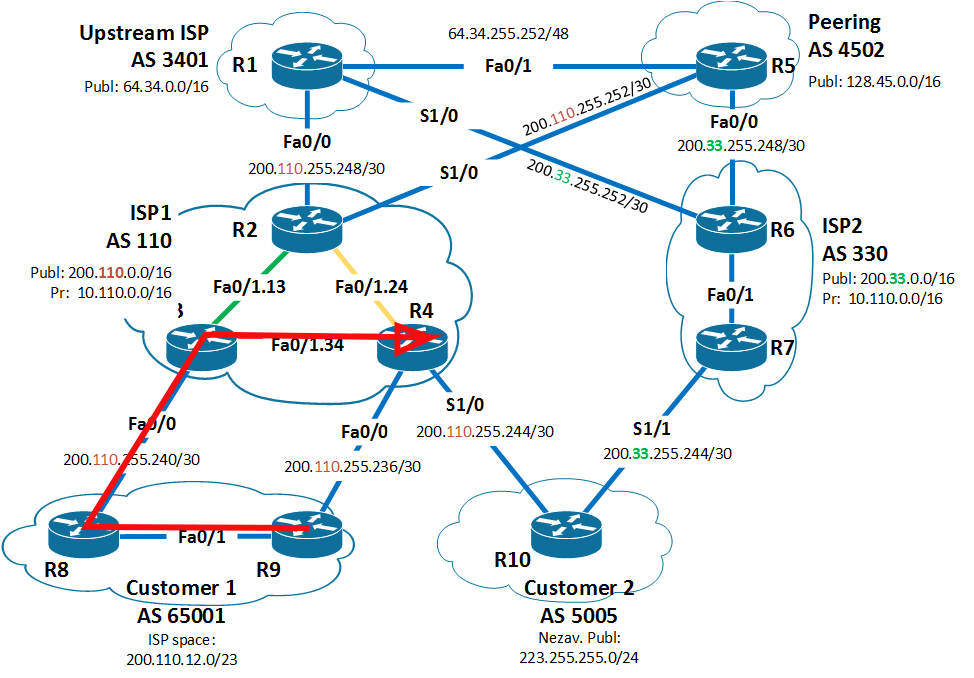
\includegraphics[width=14cm,keepaspectratio]{bgp_isis_r3_r8_primary}
\caption{Topológia BGP}
\label{fig:bgp_isis_topo_r3_r8}
\end{figure}

\newpage

\subsubsection{Konfigurácia}
\paragraph{}

\noindent
{\fontfamily{qcr}\selectfont
\begin{small}
\begin{alltt}
=============================================================
!SMEROM VON
=============================================================

!R8
conf t
!Nastavenie priority pre R3 smerom von
route-map PREFER permit 10
  set local-preference 110
router bgp 65001
  neighbor 200.110.255.241 route-map PREFER in
end
clear ip bgp * in



-------------------------------------------------------------


!R9
ip bgp-community new-format
route-map OUT permit 10
  set community 65001:110
router bgp 65001
  neighbor 200.110.255.237 route-map OUT out
  neighbor 200.110.255.237 send-community
end
clear ip bgp * out


-------------------------------------------------------------


!R3, R4
ip bgp-community new-format






=============================================================
!SMEROM DNU
=============================================================

!R3
!vytvoríme ACL pre komunitu
ip community 1 permit 65001:110

route-map CUSTOMER permit 10
  match community 1
  set local-preference 110
router bgp 110
  neighbor 200.110.255.242 route-map CUSTOMER in
end
clear ip bgp * in
\end{alltt}
\end{small}
}

\subsubsection{Overenie}
\paragraph{}

\noindent
{\fontfamily{qcr}\selectfont
\begin{small}
\begin{alltt}
smerom von - od Customera 1
!R8 alebo R9
show route-map
traceroute 10.255.255.1

PREDTYM
!R9 - sledovat next hop na R1 loop
show ip bgp 


!R2
smerom dnu - do Customera 1
show ip bgp
traceroute 10.255.255.8
show ip bgp 10.255.255.8
\end{alltt}
\end{small}
}







\subsection{Primárna linka R4−R10}
\subsubsection{Popis}
\paragraph{}
Záklazník 2 chce primárne využívať linku ku R4 pre vstup aj výstup t.j. ping z R5 na R7 nepôjde cez AS 330 (R5 -\textgreater{} R6 -\textgreater{} R7), ale cez \textbf{R5 -\textgreater{} R2 -\textgreater{} R4 -\textgreater{} R10 -\textgreater{} R7}. Rovnako aj v spätnom smere.

\begin{figure}[!htbp]
\centering
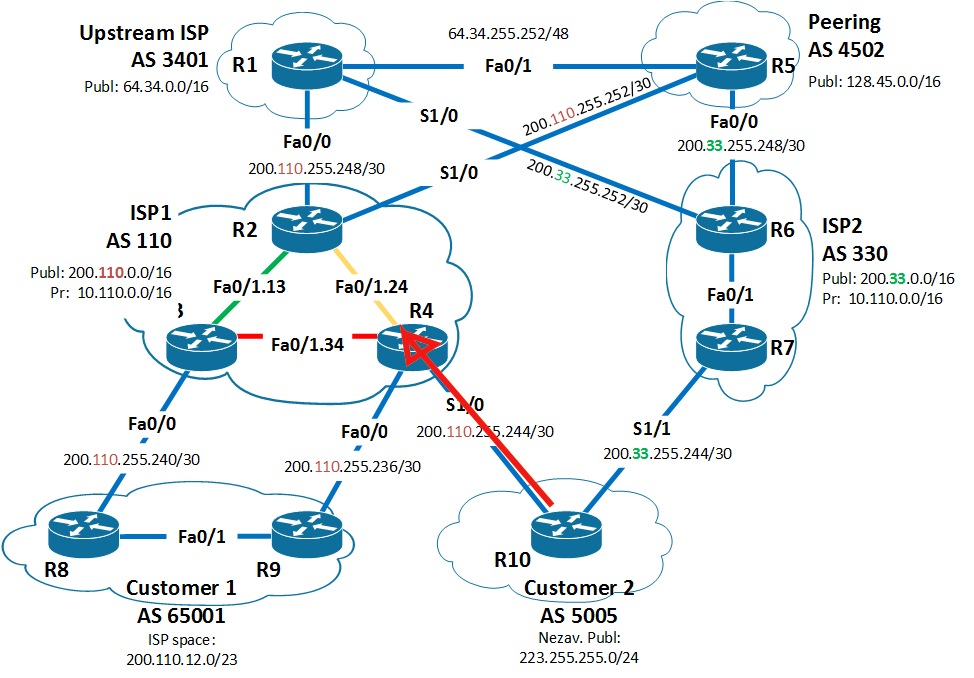
\includegraphics[width=14cm,keepaspectratio]{bgp_isis_r4_r10_primary}
\caption{Topológia BGP}
\label{fig:bgp_isis_topo}
\end{figure}

\subsubsection{Konfigurácia}
\paragraph{}
Konfigurujeme smerovač R7.

\noindent
{\fontfamily{qcr}\selectfont
\begin{small}
\begin{alltt}
=============================================================
!SMEROM VON
=============================================================

!R7
route-map ROUTE1 permit 10
  match as-path 1
  match community 2
  set local-preference 65
exit
router bgp 330
neighbor 200.33.255.246 route-map ROUTE1 in


=============================================================
!SMEROM DNU
=============================================================

R6(config)#route-map R1-R6 permit 10
R6(config-route-map)#set local-preference 60
R6(config-route-map)#exit
R6(config)#route-map R5-R6 permit 10
R6(config-route-map)#set local-preference 70
R6(config-route-map)#exit
R6(config)#router bgp 330
R6(config-router)#neighbor 200.33.255.249 route-map R5-R6 in
R6(config-router)#neighbor 200.33.255.253 route-map R1-R6 in


-------------------------------------------------------------


!R2
route-map R1-R2 permit 10
  set local-preference 60
route-map R5-R2 permit 10
  set local-preference 70
router bgp 110
  neighbor 200.110.255.249 route-map R1-R2 in
  neighbor 200.110.255.254 route-map R5-R2 in


-------------------------------------------------------------


!R10
route-map R4PREF permit 10
  set local-preference 160
router bgp 5005
  neighbor 200.110.255.245 route-map R4PREF in


-------------------------------------------------------------


!R5
route-map R1LP permit 10
  set local-preference 60
router bgp 4502
  neighbor 64.34.255.253 route-map R1LP in


-------------------------------------------------------------


!R8
route-map R3-R8 permit 10
  set local-preference 110
router bgp 65001
  neighbor 10.255.255.9 route-map R3-R8 out
\end{alltt}
\end{small}
}



\subsubsection{Overenie}
\paragraph{}
Mozme si vsimnut ze prevadzka ide cez R6.

\noindent
{\fontfamily{qcr}\selectfont
\begin{small}
\begin{alltt}
R7#sh ip bgp
BGP table version is 23, local router ID is 10.255.255.7
Status codes: s suppressed, d damped, h history, * valid, > best, 
              i - internal, r RIB-failure, S Stale
Origin codes: i - IGP, e - EGP, ? - incomplete

   Network          Next Hop        Metric LocPrf Weight Path
*>i10.255.255.1/32  10.255.255.6         0    100      0 3401 i
*>i10.255.255.2/32  10.255.255.6         0    100      0 4502 110 i
*>i10.255.255.3/32  10.255.255.6         0    100      0 3401 110 i
*>i10.255.255.4/32  10.255.255.6         0    100      0 4502 110 i
*>i10.255.255.5/32  10.255.255.6         0    100      0 4502 i
r>i10.255.255.6/32  10.255.255.6         0    100      0 i
*> 10.255.255.7/32  0.0.0.0              0         32768 i
*>i10.255.255.8/32  10.255.255.6         0    100      0 4502 110 65001 i
*>i10.255.255.9/32  10.255.255.6         0    100      0 4502 110 65001 i
*>i10.255.255.10/32 10.255.255.6         0    100      0 3401 110 5005 i
*>i64.34.0.0/16     10.255.255.6         0    100      0 3401 i
*>i128.45.0.0       10.255.255.6         0    100      0 4502 i
* i200.33.0.0/16    10.255.255.6         0    100      0 i
*>                  0.0.0.0                        32768 i
s> 200.33.7.0/25    0.0.0.0              0         32768 i
*>i200.110.0.0/16   10.255.255.6         0    100      0 4502 110 i
*>i223.255.255.0    10.255.255.6         0    100      0 4502 110 5005 i
\end{alltt}
\end{small}
}




\subsection{Distribuovať iba default, AS5005 a peering prefixy do AS65001}
\subsubsection{Popis}
\paragraph{}
R1 treba oznackovat routy. neuvidim siete ktore su z R1 + uvidime default route smerom hore

\subsubsection{Konfigurácia}
\paragraph{}
route-map
* out smery dat comunitu 3401:3401
send community
susedia by mali mat komunitu

R3,R4 in - route-mapa
ak obsahujes send comunity, neposielas to dalej

\noindent
{\fontfamily{qcr}\selectfont
\begin{small}
\begin{alltt}
!R1
route-map COM permit 10
  set community 3401:65001
router bgp 3401
neighbor 200.110.255.250 send-community
neighbor 200.33.255.254 send-community
  neighbor 200.110.255.250 route-map COM out
  neighbor 200.33.255.254 route-map COM out


-------------------------------------------------------------


!R2
R2(config)#router bgp 110
  neighbor 10.255.255.3 send-community
  neighbor 10.255.255.4 send-community
do clear ip bgp * out


-------------------------------------------------------------


!R3
R3(config)#ip community-list 1 permit 3401:65001
route-map DEFAULT deny 10
  match community 1
  exit
route-map DEFAULT permit 20
router bgp 110
  neighbor 200.110.255.242 route-map DEFAULT out
  neighbor 200.110.255.242 default-originate


-------------------------------------------------------------


!R4
ip community-list 1 permit 3401:65001
route-map DEFAULT deny 10
  match community 1
  exit
route-map DEFAULT permit 20
exit
router bgp 110
  neighbor 200.110.255.238 route-map DEFAULT out
  neighbor 200.110.255.238 default-originate

R4(config-router)#do clear ip bgp * out
\end{alltt}
\end{small}
}


\subsubsection{Overenie}
\paragraph{}
na r8 neuvidim siete ktore su z R1 + uvidime default route smerom hore vo výpise príkazov \say{show ip route} a \say{show ip bgp} t.j. na R8 nevidím cestu do 10.255.255.1.

\noindent
{\fontfamily{qcr}\selectfont
\begin{small}
\begin{alltt}
B    223.255.255.0/24 [200/0] via 200.110.255.237, 00:11:22
     200.110.255.0/30 is subnetted, 2 subnets
C       200.110.255.240 is directly connected, FastEthernet0/0
i L2    200.110.255.236 [115/10] via 10.110.89.9, FastEthernet0/1
     200.110.12.0/25 is subnetted, 1 subnets
C       200.110.12.0 is directly connected, Loopback1
B    128.45.0.0/16 [200/0] via 200.110.255.237, 00:11:22
     200.110.13.0/25 is subnetted, 1 subnets
i L2    200.110.13.0 [115/10] via 10.110.89.9, FastEthernet0/1
     10.0.0.0/8 is variably subnetted, 10 subnets, 2 masks
B       10.255.255.10/32 [200/0] via 200.110.255.237, 00:11:24
C       10.255.255.8/32 is directly connected, Loopback0
i L2    10.255.255.9/32 [115/10] via 10.110.89.9, FastEthernet0/1
B       10.255.255.2/32 [200/0] via 200.110.255.237, 00:11:25
B       10.255.255.3/32 [200/0] via 200.110.255.237, 00:11:25
B       10.255.255.6/32 [200/0] via 200.110.255.237, 00:11:25
B       10.255.255.7/32 [200/0] via 200.110.255.237, 00:11:25
B       10.255.255.4/32 [200/0] via 200.110.255.237, 00:11:25
B       10.255.255.5/32 [200/0] via 200.110.255.237, 00:11:25
C       10.110.89.0/24 is directly connected, FastEthernet0/1
B    200.33.0.0/16 [200/0] via 200.110.255.237, 00:11:25
B    200.110.0.0/16 [200/0] via 200.110.255.237, 00:11:25



R8#sh ip bgp
BGP table version is 47, local router ID is 200.110.12.1
Status codes: s suppressed, d damped, h history, * valid, > best, 
              i - internal, r RIB-failure, S Stale
Origin codes: i - IGP, e - EGP, ? - incomplete

   Network          Next Hop            Metric LocPrf Weight Path
*>i10.255.255.2/32  200.110.255.237          0    100      0 110 i
*>i10.255.255.3/32  200.110.255.237          0    100      0 110 i
*>i10.255.255.4/32  200.110.255.237          0    100      0 110 i
*>i10.255.255.5/32  200.110.255.237          0    100      0 110 4502 i
*>i10.255.255.6/32  200.110.255.237          0    100      0 110 4502 330 i
*>i10.255.255.7/32  200.110.255.237          0    100      0 110 4502 330 i
*> 10.255.255.8/32  0.0.0.0                  0         32768 i
r>i10.255.255.9/32  10.255.255.9             0    100      0 i
*>i10.255.255.10/32 200.110.255.237          0    100      0 110 5005 i
*>i128.45.0.0       200.110.255.237          0    100      0 110 4502 i
*>i200.33.0.0/16    200.110.255.237          0    100      0 110 4502 330 i
*>i200.110.0.0/16   200.110.255.237          0    100      0 110 i
*>i223.255.255.0    200.110.255.237          0    100      0 110 5005 i
\end{alltt}
\end{small}
}




\subsection{AS5005 nesme byť nikdy transit}
\subsubsection{Popis}
\paragraph{}
Je nežiadúce, aby komunikácia medzi poskytovateľmi \say{ISP 1} a \say{ISP 2} prechádzala cez oblasť 5005 (Customer 2). Jednak by to bolo bezpečnostné riziko, a navyše by sme obmedzovali prenosovú rýchlosť zákazníka 2.

\subsubsection{Konfigurácia}
\paragraph{}

\noindent
{\fontfamily{qcr}\selectfont
\begin{small}
\begin{alltt}
!R10
route-map OUT_110 permit 10
  match as-path 1
  et community 5005:110
route-map OUT_330 permit 20
  match as-path 1
  set community 5005:330
router bgp 5005
  neighbor 200.110.255.245 route-map OUT_110 out
  neighbor 200.33.255.245 route-map OUT_330 out

\end{alltt}
\end{small}
}

\subsubsection{Overenie}
\paragraph{}
TODO - overit transit






\subsection{Peering iba pre ISP1 a ISP2, nie pre prefixy naučené z Upstream ISP}
\subsubsection{Popis}
\paragraph{}
R2 nebude ohlasovat updaty z R1 do R5
R6 nebude ohlasovat updaty z R1 do R5

\subsubsection{Konfigurácia}
\paragraph{}
TODO - na routri R5 nesedi konfiguracia routemap!

\noindent
{\fontfamily{qcr}\selectfont
\begin{small}
\begin{alltt}
TODO - Treba konkretne prikazy
R2 route map na R5
match 3401 -> deny

R6 route map na R5
match 3401 -> deny
match comunity 3401 deny
\end{alltt}
\end{small}
}

\paragraph{}
problem bol ze ked siel ping z napr R10 na R1 tak siel cez R4 R2 R5 R6 R1
treba zadat tieto prikazy aby to slo priamo do R1

\noindent
{\fontfamily{qcr}\selectfont
\begin{small}
\begin{alltt}
R2(config)#route-map DENYR1 deny 10
R2(config-route-map)#match community 1
R2(config)#route-map DENYR1 permit 20
router bgp 110
 neighbor 200.110.255.254 route-map DENYR1 out
clear


R6
ip community-list 1 permit 3401:65001
route-map DENYR1 deny 10
 match community 1
route-map DENYR1 permit 20
router bgp 330
 nei 200.33.255.249 route-map DENYR1 out
do clear ip bgp * out
\end{alltt}
\end{small}
}

\paragraph{}
teraz bol problem ze ping siel od R10 do R4 R2 R5 R1
preto bolo treba zadat do R2 takuto route-mapu

\noindent
{\fontfamily{qcr}\selectfont
\begin{small}
\begin{alltt}
!R2
route-map R1-R2 permit 5
 match community 1
 set local-preference 110
\end{alltt}
\end{small}
}

\subsubsection{Overenie}
\paragraph{}
TODO - traceroute od R10 do R4 R2 R5 R1

\end{document}